\documentclass[a4paper,12pt,twoside]{scrreprt}
% Autor der Vorlage: Klaus Rheinberger, FH Vorarlberg, 2017-02-20

% Pakete:
\usepackage[utf8]{inputenc}
\usepackage[T1]{fontenc} % Silbentrennung bei Sonderzeichen
\usepackage{graphicx} % Bilder einbinden
\usepackage{wrapfig} % Bilder positionieren
\usepackage[ngerman]{babel} % Deutsche Sprachanpassungen
\usepackage{minted} % Code Highlighting/Import
\usepackage{csquotes} % Anführungszeichen und Zitieren
\usepackage{acronym} % Abkürzungsverzeichnis
\usepackage[bindingoffset=8mm]{geometry} % Bindeverlust von 8mm einbeziehen
\usepackage{caption} % Abbildungslegenden
\usepackage{xcolor} % Farbige Hervorhebungen
\usepackage{setspace} % Zeilenabstand
\usepackage[style=authoryear,citestyle=authoryear,backend=biber]{biblatex} % Literaturverweise
\usepackage[linktocpage=true]{hyperref} % Links -> \href{https://www.wikibooks.org}{Wikibooks home}

% Einstellungen:
\captionsetup{format=hang, justification=raggedright}
\addbibresource{Zotero.bib}
\setcounter{secnumdepth}{4}
\setcounter{tocdepth}{4} % Tiefe der Gliederung im Inhaltsverzeichnis

% Custom Commands
\renewcommand{\listingscaption}{Quellcode}
\renewcommand\listoflistingscaption{Quellcodeverzeichnis}

% Dokumentenbeginn
\begin{document}
\onehalfspacing % Zeilenabstand 1,5

% Sperrvermerkseite
\thispagestyle{empty}

\section*{Sperrvermerk}
\label{sec:sperrvermerk}
Auf Wunsch der Firma Fusonic GmbH, im Auftrag der Viterma Handels GmbH, ist die vorliegende Arbeit bis zum [DATUM] für die öffentliche Nutzung zu sperren.

Veröffentlichung, Vervielfältigung und Einsichtnahme sind ohne ausdrückliche Genehmigung der oben genannten Firma und dem Verfasser nicht gestattet. Der Titel der Arbeit sowie das Kurzreferat/Abstract dürfen jedoch veröffentlicht werden.

\vspace{3cm}

\noindent Dornbirn, am [Datum] \hfill Unterschrift des Verfassers (Dominic Luidold)

\vspace{2cm}

\hfill Firmenstempel\hspace{2cm}

% Titelblatt:
% \newpage\mbox{}\newpage
\cleardoublepage   % force output to a right page
\thispagestyle{empty}
\begin{titlepage}
    \begin{flushright}
    
\includegraphics[width=0.4\linewidth]{images/Logo_FHV.jpg}
    \end{flushright}
    \begin{flushleft}
    \section*{[Titel der Arbeit]}
    \subsection*{[Untertitel der Arbeit]}
    \vspace{1cm}

    Bachelorarbeit I\\
    zur Erlangung des akademischen Grades
    \vspace{0.5cm}

    \textbf{Bachelor of Science in Engineering (BSc)}

    \vspace{1cm}
    Fachhochschule Vorarlberg\newline
    Informatik – Software and Information Engineering

    \vspace{0.5cm}

    Betreut von\newline
    Prof. (FH) Dipl. Inform. Thomas Feilhauer

    \vspace{0.5cm}

    Vorgelegt von\newline
    Dominic Luidold\newline
    Dornbirn, [Datum]
    \end{flushleft}
\end{titlepage}

% Widmung:
\newpage
\section*{Widmung}
\label{sec:widmung}
Trotz des Sperrvermerks, an der diese Arbeit gebunden ist, möchte ich es mir nicht nehmen lassen, den Personen einen Dank auszusprechen, die mich bei der Umsetzung und Realisierung meiner Bachelorarbeit I unterstützt haben.

\medskip

Zu Beginn möchte ich meinen Betreuern Thomas Feilhauer (Fachhochschule Vorarlberg) und Michael Zangerle (Fusonic GmbH) danken, die jederzeit ein offenes Ohr für Fragen, Anliegen und Unklarheiten hatten. Durch ihre fachliche Kompetenz, ihre langjährige Erfahrung sowie ihr Know-how konnte ich vieles lernen, das ich in mein weiteres Berufsleben mitnehmen kann.

\medskip

Als nächstes möchte ich meiner gesamten Familie danken, denen ich während des Schreibens dieser Arbeit wahrscheinlich mehr als nur einmal auf die Nerven gegangen bin. Nur durch die Tatkräftige Unterstützung mit Snacks, Süßigkeiten und dem besten Zimmerservice der Welt konnte ich so ungestört an der Bachelorarbeit schreiben. Ohne ihr Korrekturlesen wären zudem mehr Tippfehler vorhanden als mir lieb sind und ich auf meine Tastatur schieben kann.

\medskip

Zu guter Letzt möchte ich meine Arbeit all jenen widmen, die für die Gleichbehandlung und Gleichberechtigung aller kämpfen, sich für eine Sache einsetzen, die größer als sie selbst ist und für die sie teilweise sogar ihr Leben aufs Spiel setzen. Auch 2020 braucht es weltweit immer noch laute Stimmen - Stimmen, die sich nicht unterkriegen lassen.

\bigskip

\begin{quote}
    \begin{flushright}
        \textit{\enquote{The time is always right to do what is right.}}\\
        Dr. Martin Luther King Jr.
    \end{flushright}
\end{quote}

% Kurzreferat:
\newpage
\section*{Kurzreferat}
\label{sec:kurzreferat}

\subsection*{[Deutscher Titel Ihrer Arbeit]}

[Text des Kurzreferats]

% Abstract:
\newpage
\section*{Abstract}
\label{sec:abstract}

\subsection*{[English Title of your thesis]}

[text of the abstract]

% Vorwort:
\newpage
\section*{Vorwort}
\label{sec:vorwort}

Der Verfasser der vorliegenden Arbeit bekennt sich zu einer geschlechtergerechten Sprachverwendung.

Um die Lesbarkeit zu gewährleisten und zugunsten der Textökonomie werden die verwendeten Personen beziehungsweise Personengruppen fix männlich oder weiblich zugeordnet. Zum Beispiel wird immer \enquote{die Entwicklerin} und \enquote{der Benutzer} verwendet. Es wurde besonders darauf geachtet, stereotype Rollenbeschreibungen zu vermeiden. Die insgesamt eventuell dadurch hervorgerufene Irritation bei den Lesenden ist gewünscht und soll dazu beitragen, eine Bewusstheit für die bestehende, Frauen diskriminierende Sprachgewohnheit (generelle Verwendung der männlichen Begriffe für beide Geschlechter) zu wecken beziehungsweise zu stärken.

% Inhaltsverzeichnis:
\cleardoublepage % force output to a right page
\tableofcontents

\clearpage
\phantomsection
\addcontentsline{toc}{chapter}{Abbildungsverzeichnis}
\listoffigures

\clearpage
\phantomsection
\addcontentsline{toc}{chapter}{Quellcodeverzeichnis}
\listoflistings

\clearpage
\phantomsection
\addcontentsline{toc}{chapter}{Tabellenverzeichnis}
\listoftables

% Abkürzungsverzeichnis:
\clearpage
\phantomsection
\addcontentsline{toc}{chapter}{Abkürzungsverzeichnis}
\chapter*{Abkürzungsverzeichnis}
\begin{acronym}
 \acro{BLS}{Better Life System}
 \acro{CI}{Continuous Integration}
 \acro{CD}{Continuous Deployment}
 \acro{CQRS}{Command Query Responsibility Segregation}
 \acro{CRUD}{Create, Read, Update, Delete}
 \acro{DTO}{Data Transfer Object}
 \acro{IDE}{Integrierte Entwicklungsumgebung}
 \acro{LTS}{Long Term Support}
\end{acronym}

\chapter{Einleitung}
\label{chap:einleitung}
Diese Bachelorarbeit verfolgt das Ziel, einen Einblick in die Implementierung und Erweiterung des bereits bestehenden Backend-Systems des \enquote{Better Life System} (kurz \enquote{BLS}) der Viterma Handels GmbH mit dem sogenannten \enquote{CQRS}-Pattern zu geben.

Das Better Life System - welches von Fusonic GmbH entwickelt wird und mittels einer Weboberfläche und gängigen Webbrowsern bedient werden kann - ermöglicht es Endkunden, mithilfe einer Handelsvertreterin der Firma Viterma (beziehungsweise mit einer Vertreterin eines ihrer Franchise-Partner) ein Badezimmer anhand der jeweiligen Bedürfnisse auszusuchen und zu konfigurieren, um sich schlussendlich ein entsprechendes Angebot dafür erstellen zu lassen.

\section{Arbeitgeber Fusonic GmbH}
\label{sec:arbeitgeber}
Die Fusonic GmbH hat ihren Firmensitz in Götzis, Vorarlberg, und besteht aus einem Team von aktuell mehr als 25 Angestellten, Softwareentwicklerinnen und Projektleiterinnen. Diese sind aufgeteilt in diverse kleinere Teams, die intern unter anderem \enquote{Duck-Team} beziehungsweise \enquote{Parrot-Team} genannt werden. Die Teams arbeiten dabei an jeweils eigenständigen Projekten und setzen diverse Technologien ein. Zu den verwendeten Technologien gehören unter anderem C\# mit .NET, PHP mit Symfony und JavaScript/TypeScript mit Angular. \parencite[vgl.]["Übersicht aller Technologien"]{fusonic_gmbh_web_nodate} Während es  regelmäßigen Austausch unter den Teams gibt, besteht jedes aus Frontend- sowie Backend-Entwicklern, da die meisten Projekte - aufgrund der zugrundeliegenden Anwendungsfälle - aus einem Web-Frontend sowie serverseitgen Backend bestehen.

\section{Nutzung \& Umfeld des \enquote{Better Life System}}
\label{sec:nutzung-umfeld}
Die Hauptaufgabe des Better Life System liegt darin, als computergestütztes und plattformunabhängiges Tool, Vertreterinnen rund um die Viterma Handels GmbH bei der Konfiguration und Zusammenstellung eines Badezimmers - zusammen mit dem Endkunden (meist Haus- beziehungsweise Wohnungsbesitzer oder Hotels) - zu unterstützen und diesen Vorgang zu erleichtern. Das BLS wird des Weiteren dazu verwendet, aktuelle und abgeschlossene Angebote zu verwalten, Produkte, Produktinformationen und dazugehörige Preisaufschläge zu pflegen und Kundendaten abzulegen. Zudem dient es als Kontrollinstanz für in Auftrag gegebene Sanierungen, um sicherzustellen, dass alle benötigten Materialen und Teile in entsprechenden Mengen vorhanden und kompatibel sind.

Die Nutzung des BLS findet zu großen Teilen auf mobilen Rechnern beziehungsweise Laptops statt, die während der Beratung und Betreuung von Kunden zum Einsatz kommen. Da nicht immer gewährleistet werden kann, dass eine aufrechte Internetverbindung besteht, ist die Offline-Fähigkeit bei gleichbleibender Nutzung im Webbrowser ein wichtiger Bestandteil des Web-Frontends.

Aufgrund der Anforderungen der Viterma Handels GmbH, dass das Better Life System offline ebenso wie online verwendet werden kann, basiert das Frontend auf dem TypeScript Web-Framework Angular\footnote{\href{https://angular.io/}{Angular (https://angular.io)}}, welches solch eine Funktionalität ohne eine Installation oder zusätzliche Voraussetzungen am Endgerät unterstützt. Im Gegensatz zu weniger komplex gehaltenen Frontends - die primär Daten darstellen, die vom Backend eingehen - ist dieses beim BLS für einen Großteil der Ablauflogik, Berechnung von Preisen und Generierung von diversen PDFs zuständig. Das Frontend wird, da der Fokus dieser Arbeit auf der Entwicklung im Backend der Anwendung liegt, in weiterer Folge jedoch nicht genauer beleuchtet und als gegeben angenommen. Es kann davon ausgegangen werden, dass eingehende Anfragen an das Backend aus Benutzereingaben beziehungsweise zeitlich gesteuerten Events resultieren.

\pagebreak

Das Backend, welches alle API-Anfragen bearbeitet und als Schnittstelle zur Datenbank dient, ist in der Programmiersprache PHP geschrieben und verwendet das Framework Symfony\footnote{\href{https://symfony.com/}{Symfony (https://symfony.com)}} sowie diverse \enquote{Bundles}, die darauf aufbauen. Ein detaillierterer Überblick über den Aufbau, bisher angewandte Konzepte sowie technische Begebenheiten werden in Kapitel~\ref{chap:stand-technik} auf Seite \pageref{chap:stand-technik} behandelt.

\medskip

Während die Nutzung des Better Life System auf allen Plattformen - die einen modernen Webbrowser anbieten - möglich ist, findet die Entwicklung primär auf der Linux-Distribution  Ubuntu statt. Der Grund für diese Betriebssystemwahl ist damit zu erklären, dass sowohl die lokale Entwicklung als auch die Continuous Integration Umgebung (genutzt für automatisierte Tests) und das Continuous Deployment mittels Docker\footnote{\href{https://docker.com}{Docker (https://docker.com)}} Containern stattfindet. Für die Entwicklung im Backend-Bereich der Anwendung wird die IDE PhpStorm verwendet, während im Frontend auf Visual Studio Code gesetzt wird.

\section{Problemstellung}
\label{sec:problemstellung}
Die Entwicklung des BLS hat im Frühjahr 2017 begonnen und die Anwendung ist seit dem stetig weiterentwickelt worden. Über die Zeit haben sich entsprechend sowohl die Anforderungen und Wünsche des Kunden als auch die technischen Begebenheiten, Best Practices und Möglichkeiten verändert.

Die bisher bei der Umsetzung des Projekts verwendete Struktur sowie der Aufbau wurde stark an die empfohlene Herangehensweise von Symfony angelehnt und die Code-Basis entsprechend darauf ausgelegt \parencite[siehe dazu][\enquote{The Symfony Framework Best Practices}]{symfony_symfony_nodate}. Durch wachsende Anforderungen und entsprechend benötigten Programmcode, der diese erfüllt, hat sich jedoch ein komplexes System ergeben, dessen \textit{Controller}, \textit{Entities}, \textit{Manager (Services)} und \textit{Data Transfer Objects (DTOs)} auf viele Verzeichnisse und Unterverzeichnisse verteilt sind. Die Abbildung~\ref{fig:ordnerstruktur} auf Seite \pageref{fig:ordnerstruktur} zeigt einen Ausschnitt von Ordnern die im Projekt vorkommen und jeweils alle Klassen ihrer Art beinhalten (im Verzeichnis \enquote{Controller} befinden sich, um ein Beispiel zu nennen, alle Controller des Projekts).

\begin{figure}[ht]
    \centering
    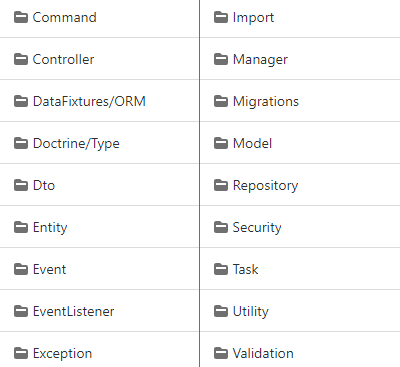
\includegraphics[scale=0.75]{images/bls_folder_structure.png}
    \caption{Teilausschnitt der BLS-Ordnerstruktur}
    \label{fig:ordnerstruktur}
\end{figure}

Durch die bisher gewählte Herangehensweise und den entsprechenden Aufbau hat sich jedoch ergeben, dass eine logische Gruppierung bzw. Kapselung von zusammengehörenden Klassen, Controllern, Managern etc. eines API Endpunkts nur schwer möglich ist. Das hat zur Folge, dass das System an manchen Stellen sehr komplex aufgebaut ist und externe Personen eine gewisse Zeit brauchen, um sich mit internen Abläufen vertraut machen zu können. Neben der Verständlichkeit ist dadurch in weiterer Folge auch die Wartbarkeit und einfache Erweiterbarkeit im Falle von neuen Funktionalitäten nicht im vollen Ausmaß gegeben. Das Testen einzelner Bestandteile mittels sogenannter \textit{Unit Tests} findet im Moment nur an wenigen Stellen statt. Primär wird beim Better Life System auf \textit{Funktionale Tests} gesetzt, die im Problemfall jedoch nur grundsätzlich darauf hindeuten können, wo ein Fehler aufgetreten ist.

Da sich die Anforderungen an das Backend auch in Zukunft noch weiterentwickeln können und eine Skalierung der Infrastruktur beziehungsweise Abspaltung einzelner Teile (in sogenannte Microservices) nicht ausgeschlossen werden kann, bedarf es Möglichkeiten, dies möglichst effektiv und ohne großen, zusätzlichen Aufwand umsetzen zu können. Die von Symfony empfohlene Herangehensweise kann dies dabei nur bedingt unterstützen, was auch in diesem Fall einen limitierenden Faktor darstellt.

\section{Anforderungen}
\label{sec:anforderungen}
Die in Abschnitt~\ref{sec:problemstellung} angeführten Umstände und den daraus resultierenden Herangehensweisen, die nicht mehr in vollem Maße zufriedenstellend sind, führen zu neuen Anforderungen an das Better Life System. Diese sollen entsprechend umgesetzt werden, um ein zukunftssicheres Backend für die gesamte Anwendung garantieren zu können und die Entwicklung neuer sowie bestehender Funktionalitäten zu erleichtern und zu vereinheitlichen.

\medskip

Zum Start des Berufspraktikums Anfang Juli 2020 stand bereits fest, dass in weiterer Folge das CQRS-Pattern (was für \textit{Command Query Responsibility Segregation} steht) zum Einsatz kommen wird. Andere Projekte der Fusonic GmbH, die primär auf C\# und .NET basieren, haben bereits gute Erfahrungen damit gemacht und gehen deshalb davon aus, dass der Einsatz Patterns die Qualität der bestehenden Code-Basis verbessern wird.

\medskip

Die Anforderungen, die im Zuge des Berufspraktikums und folglich dieser Bachelorarbeit zu erfüllen sind, bestehen darin, das aktuell bestehende System, neben dem \enquote{Tagesgeschäft} (sprich Bugfixes, Feature Requests etc.), laufend umzustellen und neue Funktionalitäten entsprechend mit der neuen Struktur und dem Pattern umzusetzen.

\section{Zielsetzung}
\label{sec:zielsetzung}
Die in den Abschnitten~\ref{sec:problemstellung} und \ref{sec:anforderungen} angeführten Punkte ergeben folgende Ziele, die im Verlauf des Berufspraktikums - so weit wie möglich - umzusetzen sind.

\smallskip

\noindent
Als Ziele einzustufen sind:
\begin{itemize}
    \item Vorbereitung der bestehenden Infrastruktur auf CQRS in Zusammenarbeit mit Mitarbeitern der Fusonic GmbH
    \item Umstellung der bestehenden API Endpunkte auf CQRS bei Beibehaltung von möglichst viel Programmlogik
    \item Umsetzung neuer Funktionalitäten mittels CQRS
    \item Weiterhin Abwickeln des Tagesgeschäftes
\end{itemize}

\chapter{Stand der Technik}
\label{chap:stand-technik}
Das folgende Kapitel gibt einen Überblick über den aktuellen Stand des Backends des Better Life System, dessen technischem Aufbau und dem zugrundeliegenden Konzept. Anschließend wird die von Symfony empfohlene Architektur beleuchtet und auf das zukünftig eingesetzte CQRS-Pattern eingegangen. Am Ende des Kapitels werden die Symfony Standard-Architektur und CQRS gegenübergestellt und Vor- sowie Nachteile aufgezeigt.

\section{Aufbau des Backends}
\label{sec:aufbau-backend}
Das Backend des BLS basiert auf der Programmiersprache PHP und setzt hierbei auf die zum aktuellen Zeitpunkt (Stand August 2020) neueste Version \textit{PHP 7.4}. Zur Verwaltung benötigter Abhängigkeiten kommt das Paketverwaltungssystem Composer\footnote{\href{https://getcomposer.org}{Composer (https://getcomposer.org)}} zum Einsatz, welches alle benötigten Symfony Bundles und anderweitige Packages sowohl im Produktivsystem als auch während der Entwicklung zur lokalen Installation sowie Nutzung zur Verfügung stellt.

Als Grundgerüst für das Backend dient das PHP-Framework Symfony in der LTS-Version \textit{4.4}, wobei zum Zeitpunkt des Verfassens dieser Arbeit Vorbereitungen für einen Umstieg auf Version \textit{5.x} getroffen werden. Das Backend dient als Schnittstelle zwischen dem Angular-Frontend und einem Datenspeicher, wobei hierfür eine relationale Datenbank auf Basis von MySQL eingesetzt wird.

\medskip

Der grundsätzliche Aufbau des Symfony Backends entspricht aktuell der empfohlenen Vorgehensweise laut Symfony Dokumentation und wird im folgenden Abschnitt~\ref{sec:symfony-aufbau} auf Seite \pageref{chap:stand-technik} erläutert.

\section{Standard Symfony Architektur}
\label{sec:symfony-aufbau}

% Literaturverzeichnis:
\clearpage
\phantomsection
\addcontentsline{toc}{chapter}{Literaturverzeichnis}
\printbibliography

\chapter*{[evtl. Anhang]}  % evtl. ersetzen mit \chapter*{Anhang}
\addcontentsline{toc}{chapter}{[evtl. Anhang]}   % evtl. ersetzen mit \addcontentsline{toc}{chapter}{Anhang}
Formatvorlage für den Fließtext.

\chapter*{Eidesstattliche Erklärung}
\addcontentsline{toc}{chapter}{Eidesstattliche Erklärung}
Ich erkläre hiermit an Eides statt, dass ich die vorliegende Bachelorarbeit I selbstständig und ohne Benutzung anderer als der angegebenen Hilfsmittel angefertigt habe. Die aus fremden Quellen direkt oder indirekt übernommenen Stellen sind als solche kenntlich gemacht. Die Arbeit wurde bisher weder in gleicher noch in ähnlicher Form einer anderen Prüfungsbehörde vorgelegt und auch noch nicht veröffentlicht.

\vspace{3cm}
\noindent
Dornbirn, am [Datum]\hfill Dominic Luidold

\end{document}
